\section{Design}

\subsection{Hardware}

Systemet består af PSoC-Master som er forbundet til DevKit8000 med et 4-ledningers SPI-bus og forbundet til PSoC-XY, -Z og -Senser med et 2-ledningers I2C-bus med eksterne pull-up modstande. Til test/debugning er der også brugt en UART forbindelse til at udlæse til Tera Term og en Nokia 5110 skærm til at aflæse indkommende og udgående kommuniaktion via SPI og I2C. På figur \ref{fig:psoc-master_topdesign} kan tilslutningerne for PSoC-Master ses.

% TopDesign PSoC-Master.
\begin{figure}[H] \centering
    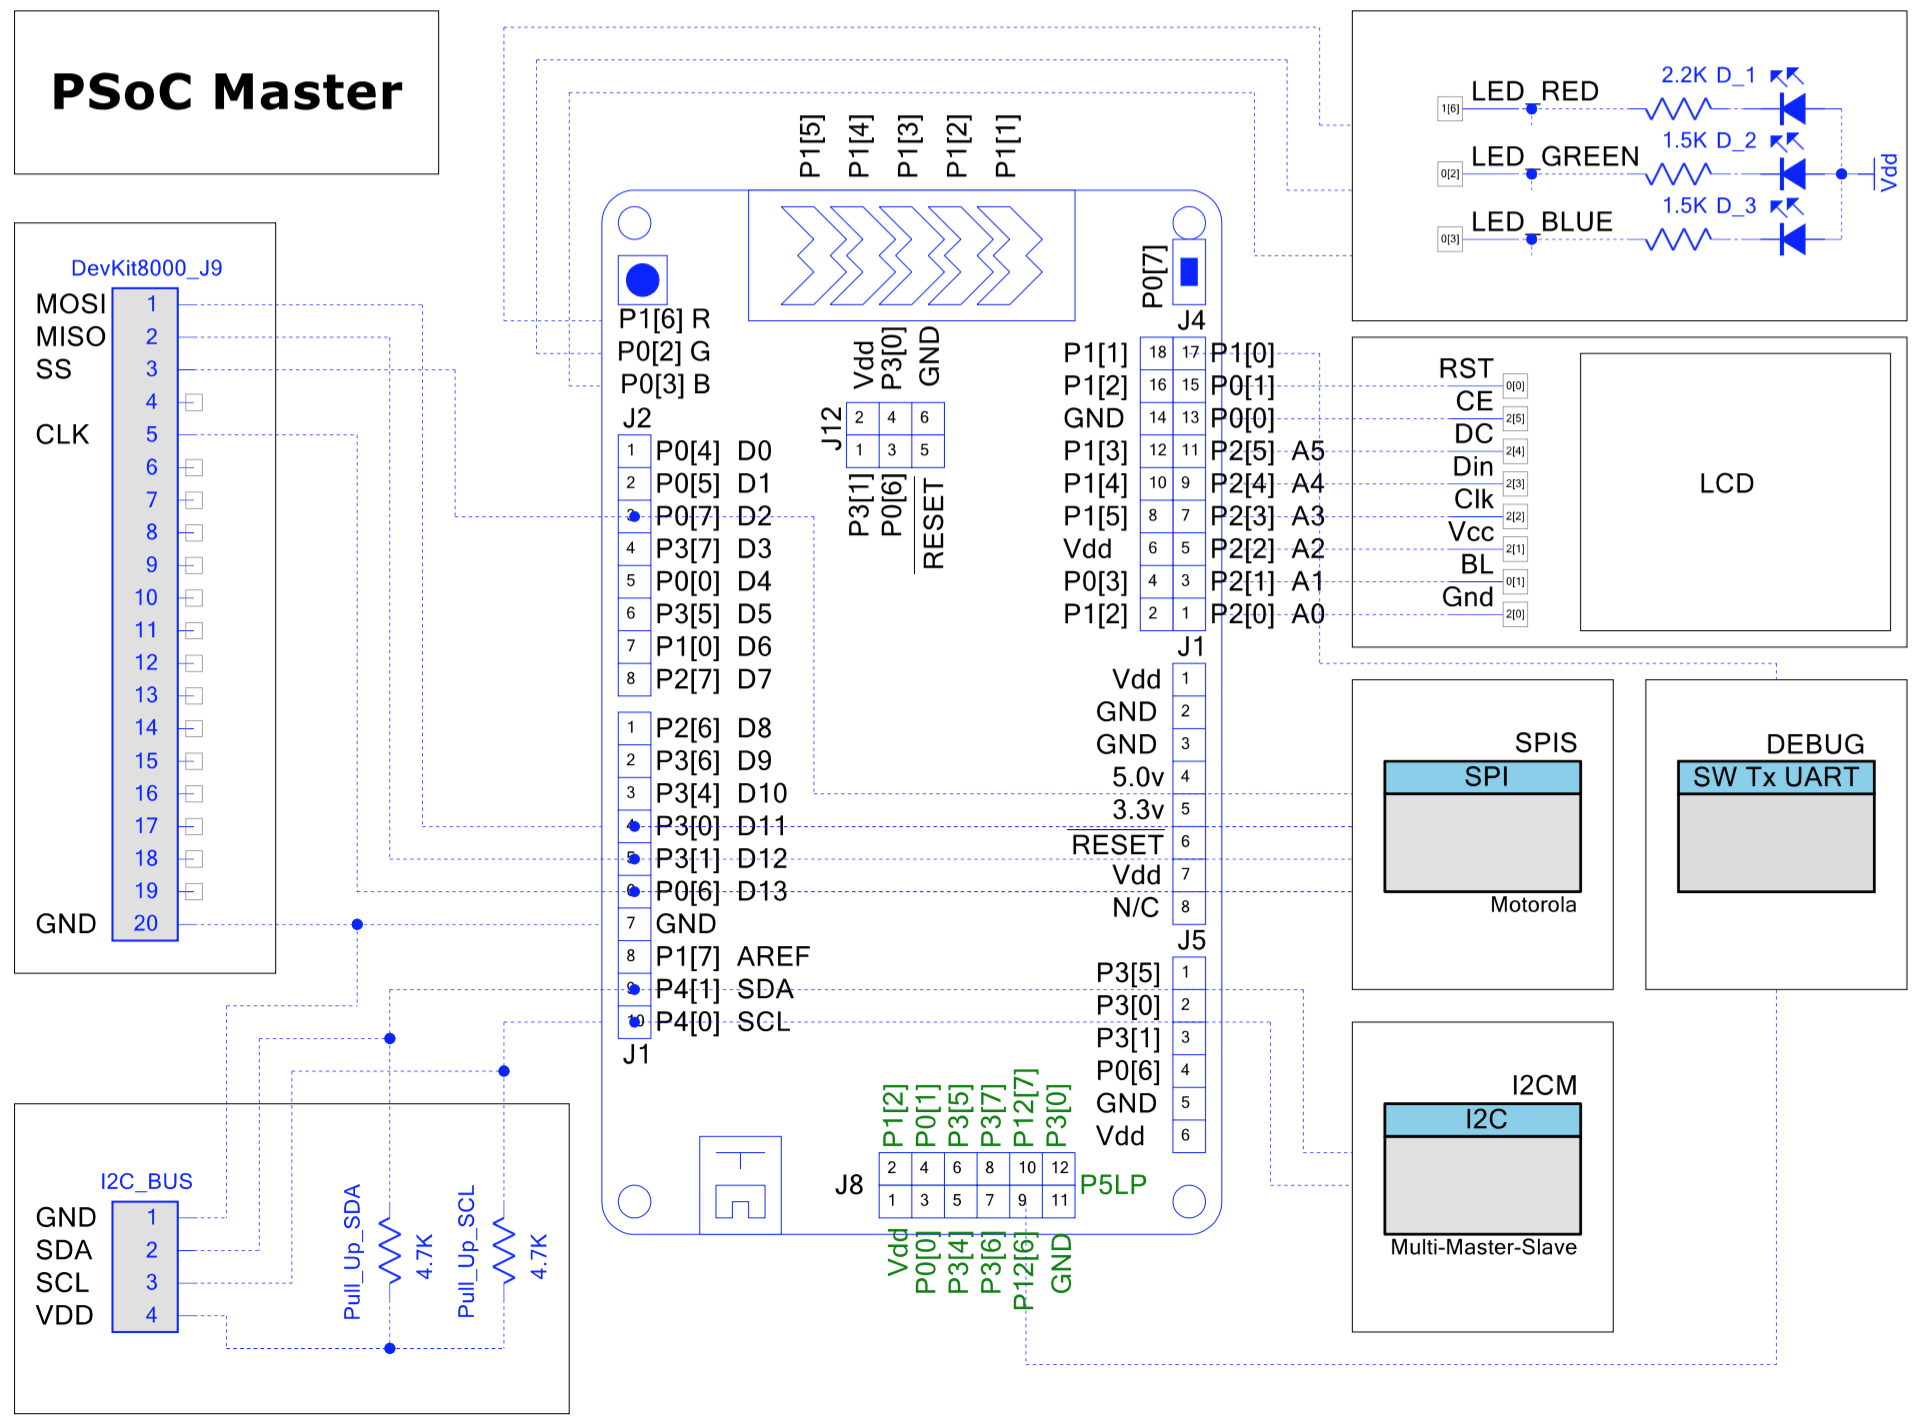
\includegraphics[width=\textwidth]{Filer/PSoC-Master_TopDesign.png}
    \caption{TopDesign PSoC-Master}
    \label{fig:psoc-master_topdesign}
\end{figure}

\subsubsection{Master-Blokken}
Systemet består af:
\begin{itemize}
	\item En PSoC.
\end{itemize}

Formålet med PSoC-Master er at den skal fungere som en "beskedcentral" mellem DevKit8000 og PSoC-XY, -Z og -Sensor.

Forbindelsen med DevKit8000 køre over SPI kommuniaktion, hvor DevKit8000 er SPI-master og PSoC-Master er SPI-slave. Når DevKit8000 sætter SS\footnote{Slave select} lav starter en ISR\footnote{Interrupt Service Routine} routine på PSoC-Master. DevKit8000 sender så via SPI-protokolen en 16-bit pakke til PSoC-Master og sætter herefter SS høj igen, for at afslutte.
PSoC-Master bearbejder herefter det modtaget 16-bit data og deler det om i to mindre stykker hhv. en kommando og en værdi.
Komandoen og værdien bliver pakket ind i en struct\footnote{data} og sat ind i en fifo\footnote{First in, first our} kø\footnote{queue}.
I hovedprogrammet på PSoC-Master bliver der løbende kontroleret om der er data i køen der skal håndteres, når dette er tilfældet, så trækker den dataen ud af køen og sender det til handleren\footnote{handler} i form af kommando og værdi. I handleren bliver der kigget på hvilken kommando der er modtaget og ud fra kommandolisten\footnote{kommandoer} bliver der fortaget den handling som hidrøere kommandoen. 

Hvis kommandoen f.eks. er at sætte en X position, så vil handleren kalde I2C-set\footnote{i2c} funktion med paremeterene for: modtagers I2C-adresse, kommando og værdi. I2C funktionen pakker den modtaget kommando og værdi ind i en buffer til I2C afsending, i buffer er der også blevet tilføjet en SOP\footnote{Start of packet} og en EOP\footnote{End of packet} som bliver send med som den første og sidst byte i kommuniaktionen. Disse bytes bliver brugt af modtageren til at kontrollerer at det modtaget data er valid.

Når kommandoen er afsendt og handleren derved er færdig med opgaven, vil vi komme tilbage til hovedprogrammet, hvor vi så fjerne dataen i køen og derefter kigger i køen igen om der er mere data der skal behandles.

\subsubsection{XY-Blokken}

Designet af XY blokken består af følgende 3 dele.

\begin{itemize}
    \item En PSoC\footcite{psoc}
    \item 4 stk. Stepper motor af typen (28BYJ-48) se databladet i bilag.
    \item 4 stk. Micro switches af typen (DM1-01P-30-3) se databladet i bilag.
\end{itemize}

For at kunne styre stepper motorerne er der implementeret en motorstyring. PSoC har 4 pins den sætter højt skiftevis, disse 4 pins giver et signal til motorstyringen, som alt efter hvilken pin der er aktiv, aktivere en spole i motoren, som så skifter polerne på en magnet, dette sker ved at den tilslutter en stel forbindelse så der kan løbe en strøm i spolen. Magneten kan ved pol skift få motoren til at bevæge sig. Ved at styre rækkefølgen af hvordan disse pins bliver sat høj kan man styre hvad vej motoren kører. Som ende stop på XY skinnerne er der blevet implementeret 4 switches/kontakter, 2 på X og 2 på Y. Kontakterne, ved aktivering, vil stoppe for den bevægelse der er i gang for at sikre systemets fortsatte drift. Yderligere bruges kontakterne ved kalibrering for at den kan registrere når lampen er nået.

\subsubsection{Z-Blokken}

Designet Z blokken består af følgende 3 dele.

\begin{itemize}
	\item En PSoC.
	\item Én Stepper motor af typen (28BYJ-48) se databladet i bilag.
	\item Én Micro switches af typen (DM1-01P-30-3) se databladet i bilag.
\end{itemize}

Motoren til Z-aksen er styret på samme måde som motorerne for XY-delen. Dvs. Motoren har 4 input pins + en 5 V Vcc. Sættes de 4 input pins gentagende skiftevis til ground, i en bestemt rækkefølge, vil motoren køre i en rundt. Vælges den modsatte rækkefølge kører motoren baglens.

Lampen hejses ned fra vognen med et fladt bånd. Køres lampen op vil den på et tidspunkt ramme en switch oppe under vognen. Til at signalere hvornår lampen er kørt langt nok ned, afhænger systemet af afstandssensoren, som sidder inde i lampen til at vurdere og markere hvornår en nedre grænse for Z-højden er nået.

\subsubsection{Sensor-Blokken}

Systemets sensorer er monteret direkte på bunden af vognen der kører på Y-aksen. Her er de forbundet til Z-vognprintet som giver det direkte forbindelse til PSoC-Sensor hvorfra de styres.

\subsection{Software}

\subsubsection{Devkit8000-Blokken}

Systemet består af:
\begin{itemize}
	\item Et Devkit8000.
\end{itemize}

Devkit8000 skal fungere som en fjernbetjening og dermed fra den at brugeren kan interagere med systemet.

Devkit8000 indeholder en grafisk brugerflade (GUI) bestående af nogle grafiske elementer oprettet fra QT's designer widgets. Disse elementer påvirkes live som eventbaseret system, og er det brugeren kan se på Devkittets touchdisplay. Når Devkittet påvirkes via touchskærmen blive kode eksekveret i baggrunden afhængigt af brugerens handlinger. Handlingerne generere nogle signaler, der internt i koden udløser noget respons ved eksekvering af metoder. Hvad enten denne respons udelukkende foregår internt på Linux platformen eller sendes videre til resten af systemet vha. SPI-kommunikation er afhængigt af givne handling brugeren udfører. Alle handlinger bliver tracket i koden vha. signalerne med nogle tilhørende debugging-koder, der oplyser programmøren om hvilken effekt givne handling havde for kodens udførsel og forløb.

Et eksempel på dette kunne være at et grafisk element bestående af en slider til styring af lampens position i x-aksen. Når denne sliders markørposition ændres vil en sliderværdi blive opdateret i koden (metoderne), som en udvalgt funktion (slot) kan benytte og enten læse fra den eller skrive til den. Jævnfør dette eksempel nøjes, der med at blive læst fra slideren og det tilhørende slot (metode) er nu oplyst om at det grafiske element er blevet påvirket, og hvad dens værdier er på nuværende tidspunkt. Dette ville være et eksempel på beskedhåndtering internt i koden. Hvis brugeren vælger at denne værdi skal videreføres til resten af systemet/produktet, kan dette blive realiseret ved tryk på en Go-knap, der videresender positioneringsdata. Den satte dataværdi fra slideren bliver nu læst, behandlet og sendt videre jævnfør SPI-API'en. Hvis kommunikationen sker fejlfrit vil PSoC Master videredistribuere data, og lampen vil bevæge sig. Hvis kommunikationen fejler vil fejlkoder blive returneret til Devkit8000.

\subsubsection{Master-Blokken}
PSoC-Masters software er delt op i følgende moduler

\begin{itemize}
    \item data
    \item handler
    \item i2c
    \item led
    \item main
    \item queue
    \item spi
\end{itemize}

\textbf{Data}-structen indeholder værdier indhentet fra PSoC-XY, -Z og -Sensor.
Formålet er at DevKit8000 kan få hurtig adgang til disse. Så i tilfælde af at DevKit8000 skal bruge nogle data, så vil denne først sende en "opdater værdier" kommando til PSoC-Master og derefter afvente et kort stykke tid inden den så henter disse opdateret værdier fra PSoC-Master. I mellemtiden går PSoC-Master ud til den relavante PSoC og henter de pågælende værdiere og opdatere dem i data structen, så de er klar til at DevKit8000 kan hente dem.

I \textbf{handleren} modtages to parametere hhv. kommando og værdi.
Herefter udføres der en funktion ud fra den modtaget kommandoen med den modtaget værdi.

Via \textbf{I2C} modulet sendes og hentes der pakker på I2C-busset.
For at kunne gøre dette skal modulet have parametere for modtager adressen, kommandoen- og værdien der skal sende med.

\textbf{Led} kan tænde/slukke PSoC-Masters red-, green- og blue-led. Dette bruges i forbindelse med kommunaktionen til at angive aktivitet og om pakker er blevet afsendt eller fejlet.

Hovedeprogrammet \textbf{main} intilizere modulerne og køre derefter  loop hvor der bliver kontrolieret om der er nogle actions i køen der skal håndteres af handleren.

\textbf{Queue} håndtere køen der er bygget op at en FIFO queue der bruger en linked list til at håndtere elementer med.

Modulet \textbf{spi} modtager og håndter data pakker fra DevKit8000 og opdatere data i SPI bufferen til aflæsning fra DevKit8000.

t til ende på den pågældende skinne.  

\subsubsection{XY-Blokken}

Dele af PSoC-XY softwaren er opbygget med samme moduler som på PSoC-Master, herunder modulerne data, handler, led, main og queue.

Der er ydermere tilføjet/ændret disse moduler
\begin{itemize}
    \item data
    \item i2c
    \item led
    \item xy
\end{itemize}

\textbf{Data} modulet håndtere værdierne for XY såsom den nuværende position, max position, er enheden kalibreret og hvilken vej køre enheden.

\textbf{I2C} modtager data pakker fra PSoC-Master og bearbejder dem til en action som indsættes i køen til håndtering i hovedeprogrammet.

\textbf{Led} kan tænde eller slukke PSoC-XYs leds, dette bruges til at indikeret om PSoC-XY'en er i gang med at udføre en opgave, kalibere eller modtager et interrupt.

Modulet \textbf{xy} håndtere funktionaliteten til hardwaren og bliver kaldt fra handleren med en pågælden opgave. Ydermere håndtere den de interrups der kan forkomme fra hardwaren. 



\subsubsection{Z-Blokken}

PSoC-Zs software er stort set identisk med PSoC-XY, dog er xy-modulet udskiftet med et z-modul som er tilpasset hardwaren på PSoC-Z.


\subsubsection{Sensor-Blokken}

På TopDesign niveau består PSoC-Sensor af 7 blokke, hvoraf de mest interessante er:

\begin{itemize}
	\item Afstandssensor
	\item LED PWM
	\item Main lop metronom
	\item Debug
\end{itemize}

For at aflæse afstandssensoren skal der kunne måles hvor længe en pin bliver holdt høj, med en præcision på et par mikrosekunder (1 cm svare til 58 us). Derfor er der sat en timer op med en 1 MHz clock, der starter med at tælle på rising edge af det signal der skal måles, og derefter stopper, gemmer tællerværdien og starter en interrupt på falling edge.

Denne blok har desuden tre ekstra pins: DistTrigger, DistReset, og DistInterruptPin. DistTrigger bruges til at starte målingen - sensoren skal have en 10 us puls som input før den starter. DistReset bruges til at resette timeren mellem målingerne, da den ellers blot fortsætter med at tælle derfra hvor den kom til. Til sidst bruges DistInterruptPin til at sende et signal direkte til PSoC-Z når afstandssensoren måler at vi er kommet for tæt på en underliggende forhindring.

De tre LEDs styres med PWM, og hver farve (rød, grøn, blå) har sit eget PWM modul. De deler dog alle tre clock med afstandssensor-timeren. Dette er valgt fordi PSoC4 maksimalt understøtter fire brugerdefinerede clocks, så når forskellige komponenter kan sættes til at virke med samme clock-frekvens, er der ingen grund til at bruge flere resourcer end nødvendigt.

Metronom blokken indeholder en timer der er sat til at lave et interrupt hvert halve sekund. De interrupts bliver så brugt i hovedprogrammet til at aktiverer sensoraflæsninger og andre periodiske events. Denne timer har sin egen clock (200 Hz), da det gjorde designet nemmere og lod os holde timeren på 8 bits, hvilket sparer andre resourcer i PSoC'en.

Den sidste blok er Debug. Den indeholder et UART modul, men da de to I2C moduler optager alle de dedikerede hardware kommunikationsblokke, så der bliver her brugt et software modul der kun understøter transmit.
